\documentclass[a4paper]{article}
\usepackage[affil-it]{authblk}
\usepackage[backend=bibtex,style=numeric]{biblatex}
\usepackage{amsmath,amssymb,amsfonts}
\usepackage{tikz}
\usepackage{pgfplots}
\usepackage{amsmath}
\usepackage{geometry}
\geometry{margin=1.5cm, vmargin={0pt,1cm}}
\setlength{\topmargin}{-1cm}
\setlength{\paperheight}{29.7cm}
\setlength{\textheight}{25.3cm}

\addbibresource{citation.bib}

\begin{document}
% =================================================
\title{Numerical Analysis homework IV}

\author{LI YIJIAN 3230102477
  \thanks{Electronic address: \texttt{3230102477@zju.edu.cn}}}
\affil{(Mathematics and Applied Mathematics 2302), Zhejiang University }


\date{Due time: \today}
\maketitle





% ============================================
\section*{I. Convert 477 to a normalized FPN}
Easy to see
\[
477 = (111011101)_2
\]
so
\[
477 = (1.11011101)\times 2^8
\]
\section*{II. Convert $\frac{3}{5}$ to a normalized FPN}
Easy to see
\[
\frac{3}{5} = (0.10011001\ldots)_2
\]
so
\[
\frac{3}{5} = (1.0011001\ldots)_2 \times 2^{-1}
\]


\section*{III. Prove an equation}
We know $x = 1.0 \times \beta^e$, and $e\in (L,U) \Rightarrow e+1,e-1\in[L,U]$. Then
\[
x_{R} = 1.00\ldots01 \times \beta^e \quad
x_{L} = (\beta-1).(\beta-1)(\beta-1)\ldots(\beta-1)(\beta-1) \times \beta^{e-1} \quad
\]
Both have $p$ number. Then
\[
x - x_{L} = \beta^{e-1-p+1} \Rightarrow
RHS = \beta^{e-p+1}
= x_{R} - x 
\]




\section*{IV. Two normalized FPNs adjacent to x}
We know in IEEE 754 single-precision protocol,
$x = (1.0011001\ldots)_2 \times 2^{-1}$. Then
\[
x_{L} = (1.0011001\ldots10011001)_2 \times 2^{-1} \quad
x_{R} = (1.0011001\ldots10011010)_2 \times 2^{-1}
\]
$\Rightarrow$
\[
x - x_{L} = \frac{3}{5} \times 2^{-24} \quad
x_{R} - x = x_{R} - x_{L} + x_{L} - x = 1 \times 2^{-23} - \frac{3}{5} \times 2^{-24} = \frac{2}{5} \times 2^{-24}
\]
So
\[
fl(x) = x_{R} \quad \delta = \frac{|fl(x) - x|}{|x|} = \frac{1}{3} \times 2^{-23}
\]

\section*{V. New method of rounding off number}
By the defination in the course, the unit roundoff represents the maximul round off error
around 1, where the floating number is the densest. By the new method of rounding off number
: the badest case is the number around 1 is $1 + 2^{-23}$ in IEEE-754. So
\[
\epsilon^{new}_{u} = 2^{-23} = 2\epsilon_{u}
\]


\section*{VI. Estimate the precision lost in the subtraction}
We know:
\[
\cos x = 1 - \frac{x^2}{2!} + \frac{x^4}{4!} + O(x^6)
\]
$\Rightarrow$
\[
1-\cos \frac{1}{4} = 2^{-5} + \epsilon \quad (\epsilon \ll 2^{-5})
\]
So the subtraction will lose 5 bits of precision.

\section*{VII. Symmetric Polynomials}
Method 1:
\[
1- \cos x = 2\sin^2(\frac{x}{2})
\]
Then we know near 0 $2\sin^2(\frac{x}{2})$ is small. So without the 
subtraction of two closed number. It will NOT cause a catastrophic cancellation.
\\
Method 2:
\[
1- \cos x = \frac{1-\cos^2x}{1+ \cos x} = \frac{\sin^2 x}{1+ \cos x}
\]
For the denominator, both of them are the number closed to 1, which will NOT cause a
catastrophic cancellation. Meanwhile for the numerator, it's just a square of small number,
 which also avoid a subtraction of two closed number.


\section*{VIII. Condition numbers of functions}
We know $\operatorname{cond}_{f}(x) = \bigg|\frac{f'(x)x}{f(x)}\bigg|$
\subsection*{VIII.a}
When $\alpha = 0$ the function is trivial. We only consider the case $\alpha \neq 0$
\[
\operatorname{cond}_{f}(x) = \bigg|\frac{\alpha(x-1)^{\alpha-1}x}{(x-1)^\alpha}\bigg|
= \bigg|\frac{\alpha x}{x-1}\bigg|
\]
So the condition number is large around $x = 1$.

\subsection*{VIII.b}
\[
\operatorname{cond}_{f}(x) = \bigg|\frac{\frac{1}{x}x}{\ln x}\bigg|
= \bigg|\frac{1}{\ln x}\bigg|
\]
So the condition number is large around $x = 1$.

\subsection*{VIII.c}
\[
\operatorname{cond}_{f}(x) = \bigg|\frac{e^xx}{e^x}\bigg|
= |x|
\]
So the condition number is large when $x \rightarrow \pm \infty$.

\subsection*{VIII.d}
\[
\operatorname{cond}_{f}(x) = \bigg|\frac{x\frac{-1}{\sqrt{1-x^2}}}{\arccos x}\bigg|
= \bigg|\frac{x}{\arccos x \sqrt{1-x^2}}\bigg|
\]
So the condition number is large around $x = \pm 1$.

\section*{IX. Function $f(x) = 1-e^{-x}$}
\subsection*{IX.a}
\[
\operatorname{cond}_{f}(x) = \bigg|\frac{f'(x)x}{f(x)}\bigg| = \bigg|\frac{xe^{-x}}{1-e^{-x}}\bigg| = 
\bigg|\frac{x}{e^x-1}\bigg|
\]
When $x\in(0,1]$, $\operatorname{cond}_{f}(x) = \frac{x}{e^x-1}$, besides we know $e^x \geqslant 1 + x$. Meanwhile,
$\lim\limits_{{x \rightarrow 0}} \frac{x}{e^x-1} = 1$.
So $\operatorname{cond}_{f}(x) \leqslant 1$, when $x\in [0,1]$.

\subsection*{IX.b}

We know $f_A(x) = (1 - (1+\delta_1)e^{-x})(1+\delta_2)$, and $\delta_1,\delta_2
\leqslant \epsilon_u$, so
\[
|\delta(x)| = \bigg|\frac{f_A(x) - f(x)}{f(x)}\bigg| = 
\bigg|\frac{\delta_2 - (\delta_1+\delta_2+\delta_1\delta_2)e^{-x}}{1-e^{-x}}\bigg|
\leqslant \bigg|\frac{\delta_2 + (\delta_1+\delta_2+\delta_1\delta_2)e^{-x}}{1-e^{-x}}\bigg|
\approx \bigg|\frac{\epsilon_u e^x + 2\epsilon_u}{e^x - 1}\bigg|
 = \epsilon_u\bigg|\frac{ e^x + 2}{e^x - 1}\bigg|
\]
Therefore:
\[
\operatorname{cond}_{A}(x) \leqslant \frac{|\delta(x)|}{\epsilon_u \operatorname{cond}_f(x)}
= \frac{|e^x+2|}{|x|}
\]
\begin{figure}[h]
  \centering
  \begin{tikzpicture}
    \begin{axis}[
      domain=0.01:1,     
      samples=300,
      axis lines=middle,
      xlabel={$x$},
      ylabel={condition number},
      legend style={at={(1.1,0.97)},anchor=north east},
      xmin=0, xmax=1,
      ymin=0, ymax=20      
    ]
      \addplot[thick] {x*exp(-x)/(1 - exp(-x))};
      \addlegendentry{$\operatorname{cond}_f(x)$}

      \addplot[thick, dashed] {(1 + 2*exp(-x))/(1 - exp(-x))};
      \addlegendentry{$\operatorname{cond}_A(x)$ upper bound}
    \end{axis}
  \end{tikzpicture}
  \caption{Condition numbers on $[0,1]$}
\end{figure}


when $x \to 0$, the condition number $\operatorname{cond}_A(x)\to \infty$, it's illed. In the other points
, the algorithm works.

\section*{X. Prove a lemma}
We know
\[
||A||_2 = \max_{||x||=1}||Ax||_2 = \max_{||x||=1}\sqrt{x^{*}A^{*}Ax}
\]
Attention $A^* A$ is symmetric matrix, which can be diagonalized.
Let $\{v_i\}_{1\leqslant i \leqslant n}$ be the eigen vectors of $\{\mu_i\}_{1\leqslant i \leqslant n}$ of $A^* A$ and o.n.b by the way
(eigen vectors in different eigen vector space are orthogonal).
Then every $x$ can be written as $\sum\limits_{i=1}^{n}\alpha_i v_i$, so 
\[
||A||_2 = \max_{||x||=1}\sqrt{x^{*}A^{*}Ax} = 
\max_{\sum\limits_{i=1}^{n}\alpha_i^2 = 1}\sqrt{\sum\limits_{i=1}^{n}\mu_i^2 \alpha_i^2<v_i,v_i>}
\leqslant \sigma_{max}
\]
Meanwhile 
\[
||A||_2 \geqslant \max_{1\leqslant i \leqslant n} \sqrt{v_i^*A^*Av_i} = \sigma_{max}
\]
Then $||A||_2 = \sigma_{max}$. And notice that $(A^{-1})^*A^{-1} = (AA^*)^{-1}$. Besides by linear algebra
$|\lambda E - AB| = |\lambda E - BA|$. So we know $AA^*$ has the same eigen value as $A^*A$.
Then $||A^{-1}||_2 = \frac{1}{\sigma_{min}}$, since the eigen value of $(AA^*)^{-1}$ is $\{\frac{1}{\mu_i}\}_{1\leqslant i \leqslant n}$.
So $\operatorname{cond}_2 A = \frac{\sigma_{max}}{\sigma_{min}}$. \\
If $A = A^*$, then $\exists $ unitary matrix $U$, s.t.
\[
UAU^* = diag(\lambda_1,\ldots,\lambda_n) \Rightarrow UA^*AU^* = UAU^*UAU^* = diag(\lambda_1^2,\ldots,\lambda_n^2)
\]
Then $\operatorname{cond}_2 A = \frac{|\lambda_{\max}|}{|\lambda_{\min}|}$.
\\
If $A^*A = E \Rightarrow \mu_i = 1, \forall i$, so $\sigma_{\max} = \sigma_{\min} = 1$. Then $\operatorname{cond}_2 A = 1$.
\section*{XI. Find root of a polynomial}
We know
\[
q(r) = 0 \Rightarrow r^n + \sum\limits_{i = 0}^{n-1}a_i r^i = 0
\Rightarrow \frac{\partial r}{\partial a_i}q'(r) + r^i = 0
\]
\[
\operatorname{cond}_{f}(\mathbf{x})  = ||A(\mathbf{x})||_1
= ||(a_{ij}(\mathbf{x}))||_1
= \max_{0\leqslant i \leqslant n-1}\bigg|\frac{a_i\frac{\partial r}{\partial a_i}}{r}\bigg|
= \max_{0\leqslant i \leqslant n-1}\bigg|\frac{a_ir^{i-1}}{q'(r)}\bigg|
\]
Besides for root $r$
\[
W(x) := \sum_{i=1}^{m}(x-i)
\Rightarrow 
\operatorname{cond}_{f}(\mathbf{x}) = \max_{0\leqslant i \leqslant m-1} \bigg|\frac{r^{i-1}a_i}{W'(r)}\bigg|
= \max_{0\leqslant i \leqslant m-1} \bigg|\frac{r^{i-1}a_i}{\prod\limits_{j = 1,j\neq r}^{m}(r-j)}\bigg|
\]
Specially $r = m = 20$, $\operatorname{cond}_{f}(\mathbf{x}) \approx 2.0 \times 10^{10}$. \\
$r = m = 30$, $\operatorname{cond}_{f}(\mathbf{x}) \approx 2.0 \times 10^{16}$. \\
$r = m = 40$, $\operatorname{cond}_{f}(\mathbf{x}) \approx 1.5 \times 10^{22}$. \\
Then by comparison, i see that if a question's condition is large enough,
 it's almost impossible to find a numerical algorithm that make the condition small.
\section*{XII. Given a counter example}
Choose $\beta = 10, p = 2$. Then given $1/(2/7)$.
\[
fl_p(1/fl_p(2/7)) = fl_p(1/0.29) = 3.4
\]
\[
fl_{2p}(1/fl_{2p}(2/7)) = fl_{2p}(1/0.2857) = 3.500 \rightarrow 3.5
\]
Then get a contradiction.
\section*{XIII. Accuracy of computing root in IEEE 754}
The answer is NO. \\
In IEEE 754 $\beta = 2,p = 24,L = -126,U=127$. We know at least after $[\frac{6}{\lg 2}] + 1 = 20$ steps,
we acquire the $10^{-6}$ accuracy. But the number $\in [128,129]$, expressed as 
$ (1.a_1\ldots a_{23})_2 \times 2^{7}$. The accuracy of the number is at most $2^{7-23-1} = 2^{-17}$, which
at most ensure the accuracy of 17 steps. So we can't compute the root with absolute
accuracy $< 10^{-6}$.

\section*{XIV. Explain a phenomenon}
We know, for a pair every close adjacent points, may as well $x_1 = x_0 + h$, in this interval:
\[
s(x) = a(x-x_0)^3 + b(x-x_0)^2 + c(x-x_0) + d
\]
So we have
\[
S[a,b,c,d]^T = M
\]
For the curve is continious, we know there are two line elements of S are
\[
(0,0,0,1) \quad (h^3,h^2,h,1)
\]
which is almost linear dependent when $h \to 0$, so the $\sigma_{\min} \to \infty$.
Then the condition of $S$, $\operatorname{cond}_2(S) \to \infty$, which will make the  problem illed.
Therefore will get an inaccurate result.
\end{document}